% Created 2024-09-13 vi. 12:54
% Intended LaTeX compiler: pdflatex
\documentclass[aspectratio=169, usenames,svgnames,dvipsnames]{beamer}
\usepackage[utf8]{inputenc}
\usepackage[T1]{fontenc}
\usepackage{graphicx}
\usepackage{longtable}
\usepackage{wrapfig}
\usepackage{rotating}
\usepackage[normalem]{ulem}
\usepackage{amsmath}
\usepackage{amssymb}
\usepackage{capt-of}
\usepackage{hyperref}
\usepackage{color}
\usepackage{listings}
\usepackage[spanish]{babel}
\setbeamercolor{alerted text}{fg=Blue}
\setbeamerfont{alerted text}{series=\bfseries}
\setbeamercolor{block title}{bg=structure.fg!20!bg!50!bg}
\setbeamercolor{block body}{use=block title,bg=block title.bg}
\AtBeginSubsection[]{\begin{frame}[plain]\tableofcontents[currentsubsection,sectionstyle=show/shaded,subsectionstyle=show/shaded/hide]\end{frame}}
\AtBeginSection[]{\begin{frame}[plain]\tableofcontents[currentsection,hideallsubsections]\end{frame}}
\lstset{keywordstyle=\color{blue}, commentstyle=\color{gray!90}, basicstyle=\ttfamily\small, columns=fullflexible, breaklines=true,linewidth=\textwidth, backgroundcolor=\color{gray!23}, basewidth={0.5em,0.4em}, literate={á}{{\'a}}1 {ñ}{{\~n}}1 {é}{{\'e}}1 {ó}{{\'o}}1 {º}{{\textordmasculine}}1, showstringspaces=false}
\usepackage{mathpazo}
\hypersetup{colorlinks=true, linkcolor=Blue, urlcolor=Blue}
\usepackage{fancyvrb}
\DefineVerbatimEnvironment{verbatim}{Verbatim}{fontsize=\tiny, formatcom = {\color{black!70}}}
\usepackage{pgfplots}
\usetheme{Boadilla}
\usecolortheme{rose}
\usefonttheme{serif}
\author{Francisco Delgado López}
\date{}
\title{Desarrollo de una herramienta software para la simulación de sistemas fotovoltaicos con R}
\subtitle{Trabajo de Fin de Grado}
\institute[UPM]{Universidad Politécnica de Madrid}
\beamertemplatenavigationsymbolsempty
\setbeamertemplate{footline}[frame number]
\setbeamertemplate{itemize items}[triangle]
\setbeamertemplate{enumerate items}[circle]
\setbeamertemplate{section in toc}[circle]
\setbeamertemplate{subsection in toc}[circle]
\hypersetup{
 pdfauthor={Francisco Delgado López},
 pdftitle={Desarrollo de una herramienta software para la simulación de sistemas fotovoltaicos con R},
 pdfkeywords={},
 pdfsubject={},
 pdfcreator={Emacs 29.2 (Org mode 9.6.15)}, 
 pdflang={Spanish}}
\begin{document}

\maketitle

\section{Introducción}
\label{sec:orgefd3b82}
\begin{frame}[label={sec:orgd844b05},fragile]{Objetivo principal}
 \begin{block}{Desarrollo de un paquete en \texttt{R}}
\begin{lstlisting}[numbers=left,language=r,label= ,caption= ,captionpos=b]
library(solaR2)
\end{lstlisting}
\end{block}
\end{frame}

\begin{frame}[label={sec:org08059e0},fragile]{Objetivos secundarios}
 \begin{block}{GNU Emacs}
\end{block}
\begin{block}{Paquetes de \texttt{R}}
\begin{itemize}
\item \texttt{solaR}
\item \texttt{zoo}
\item \texttt{data.table}
\item \texttt{microbenchmark}
\item \texttt{profvis}
\item \texttt{lattice}
\end{itemize}
\end{block}
\begin{block}{\LaTeX{}}
\end{block}
\begin{block}{Energía Solar Fotovoltaica}
\end{block}
\end{frame}

\section{Estado del arte}
\label{sec:org0d44322}
\subsection{Sitación actual de la generación fotovoltaica}
\label{sec:org55cfea6}
\begin{enumerate}
\item En 2022, la energía solar fotovoltaica creció un 137\% a nivel mundial.
\item Se instalaron 240 GWp de nueva capacidad, superando los 1185 GWp en total.
\item China lidera con más de 106 GWp instalados, seguido por la Unión Europea con 41 GWp.
\item La energía solar representa el 31\% de la capacidad de generación renovable global.
\item Se añadió tres veces más energía solar que eólica en 2022.
\item La Unión Europea superó a EE.UU. en desarrollo fotovoltaico.
\item España lideró el mercado europeo con 8,6 GWp instalados.
\item El Plan REPowerEU busca alcanzar 400 GWp para 2030.
\item España instaló 5.641 MWp en plantas y aumentó el autoconsumo en un 108\%.
\item El autoconsumo industrial creció notablemente, representando el 47\% del total.
\item Se adjudicaron 1.200 MW a proyectos de hidrógeno verde y agrovoltaica.
\item El sector fotovoltaico aportó 7.014 millones de euros al PIB español y generó 197.383 empleos.
\item España fabrica el 65\% de los componentes fotovoltaicos localmente y es un importante exportador.
\end{enumerate}

\subsection{Soluciones actuales}
\label{sec:org3b08931}
\begin{frame}[label={sec:org577f747}]{Soluciones actuales}
\begin{block}{\alert{PVsyst}}
\end{block}
\begin{block}{\alert{SISIFO}}
\end{block}
\begin{block}{\alert{PVGIS}}
\end{block}
\begin{block}{\alert{System Advisor Model}}
\end{block}
\end{frame}
\begin{frame}[label={sec:org5611677},fragile]{\texttt{solaR}}
 \begin{block}{Funcionamiento}
\begin{itemize}
\item Geometría solar
\item Datos meteorológicos
\item Radiación en el plano horizontal
\item Radiación en el plano del generador
\item Simulación de SFCR
\item Simulación de SFB
\item Optimización de distancias
\item Métodos de visualización
\end{itemize}
\end{block}
\end{frame}
\begin{frame}[label={sec:org41d6875},fragile]{\texttt{solaR}}
 \begin{block}{Carencias}
\begin{itemize}
\item Modularidad
\item Eficiencia y rendimiento
\item Escalibilidad
\item Manipulación de datos
\end{itemize}
\end{block}
\end{frame}

\section{Marco teórico}
\label{sec:org9ce2099}
\begin{frame}[label={sec:org1e7fc94}]{Procedimiento de cálculo}
\begin{center}
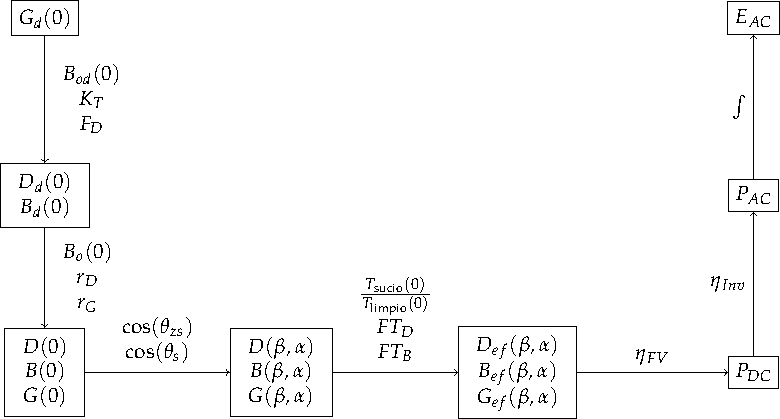
\includegraphics[scale=1]{../figuras/ProcedimientoCalculoRadiacionInclinada.pdf}
\end{center}
\end{frame}
\section{Desarrollo del código}
\label{sec:orgbcc3552}
\begin{frame}[label={sec:orge6ec4a8}]{Algorítmo de cálculo}
\begin{center}
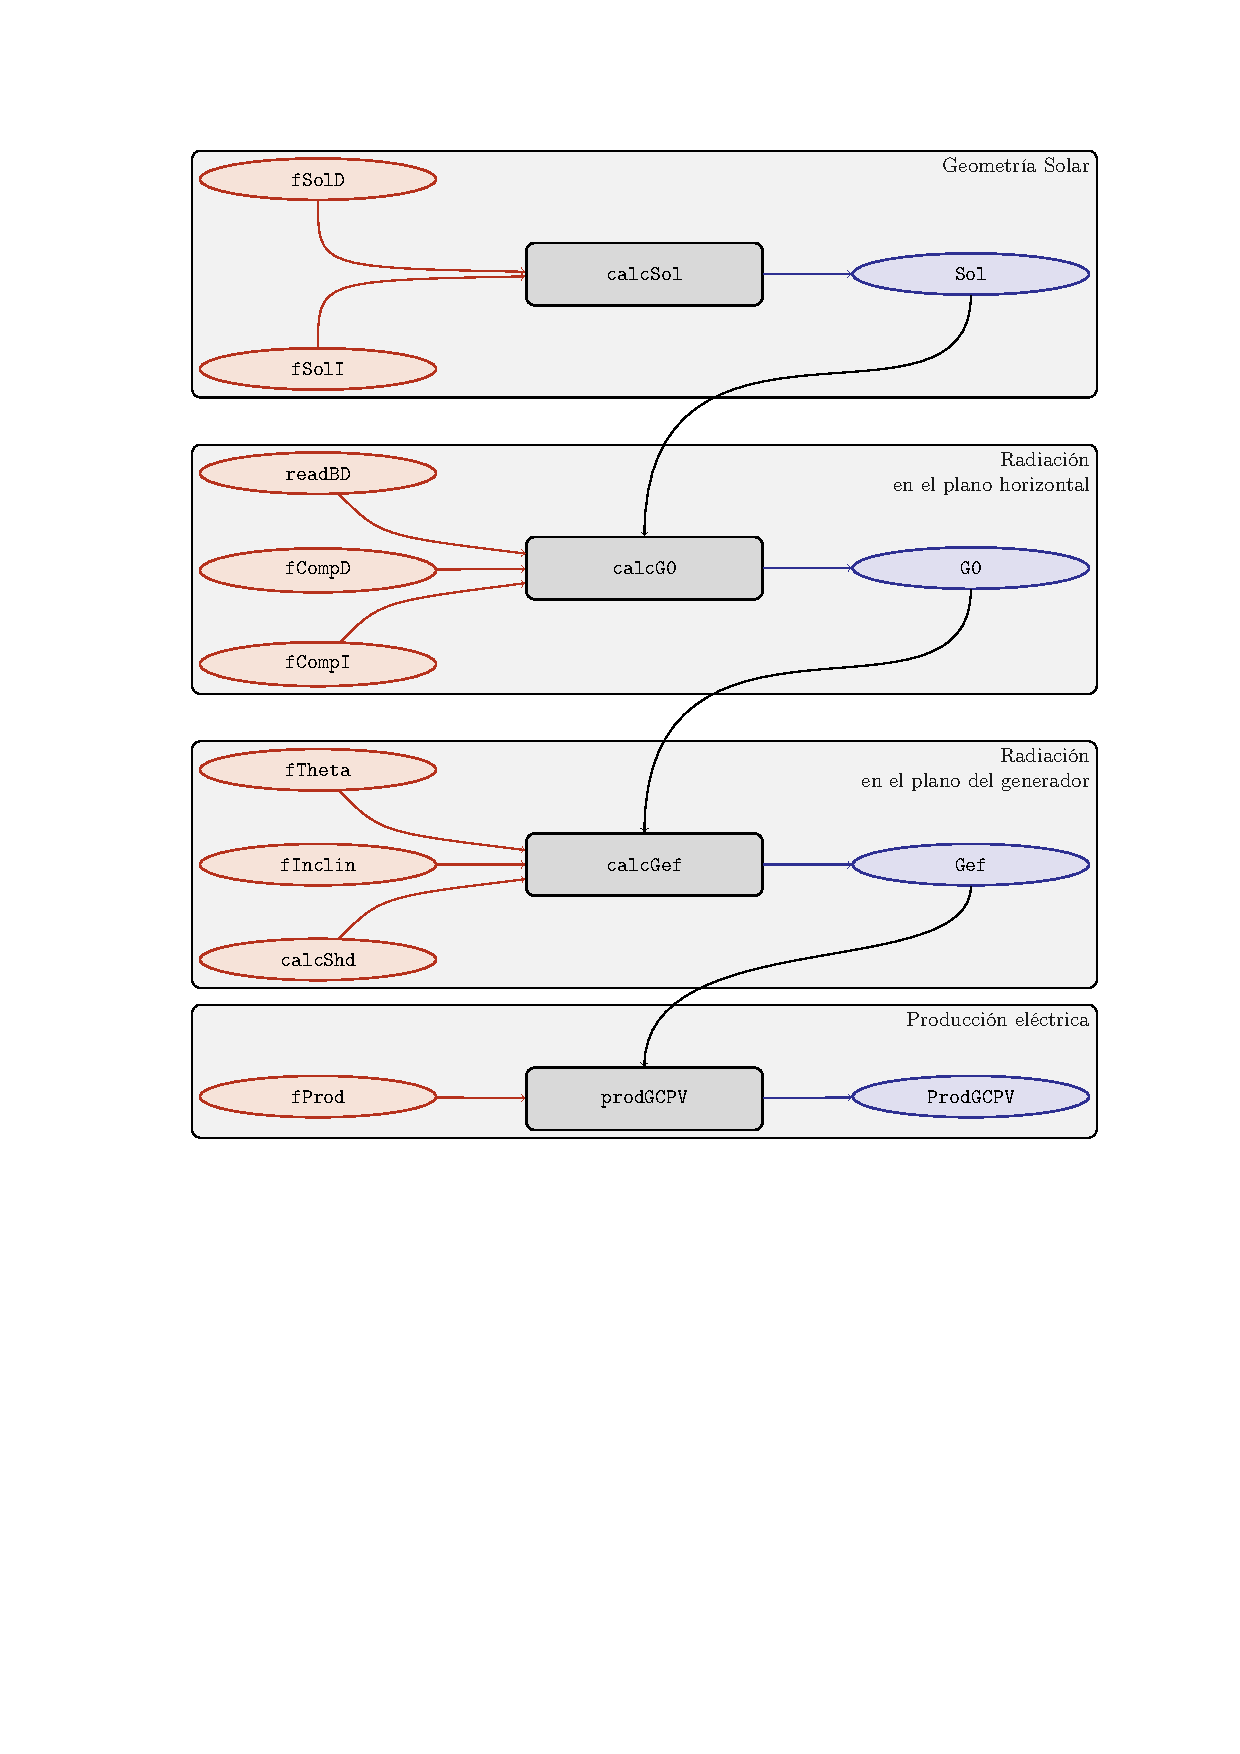
\includegraphics[height=0.9\textheight]{../figuras/procedure.pdf}
\end{center}
\end{frame}
\begin{frame}[label={sec:orgf997d71},fragile]{\texttt{calcSol}}
 \begin{center}
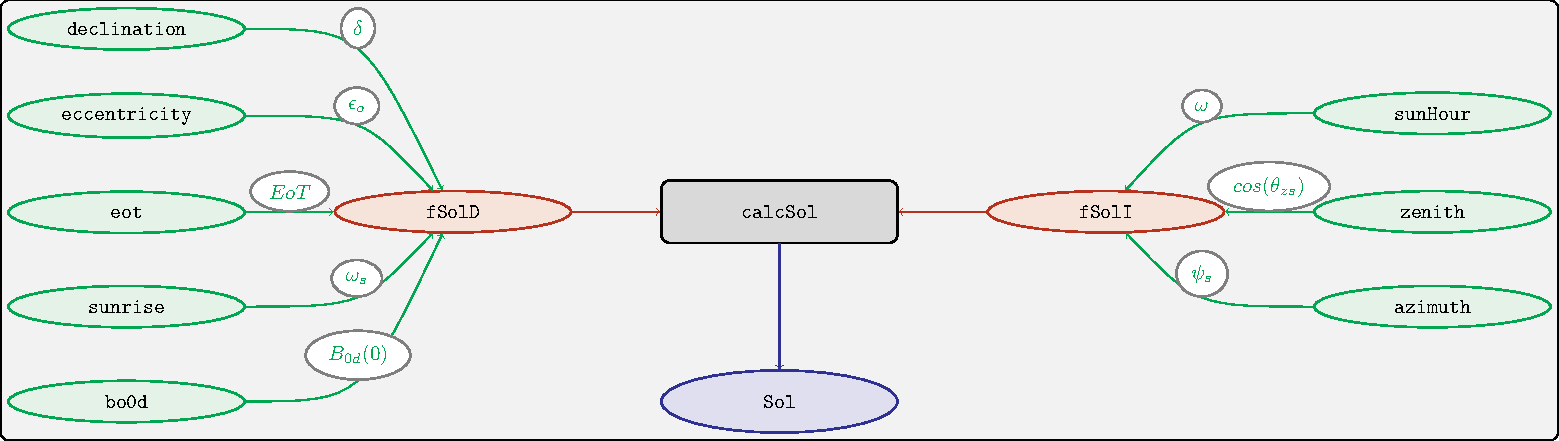
\includegraphics[width=\textwidth]{../figuras/calcsol.pdf}
\end{center}
\end{frame}
\begin{frame}[label={sec:orga8b4018},fragile]{\texttt{Meteo}}
 \begin{center}
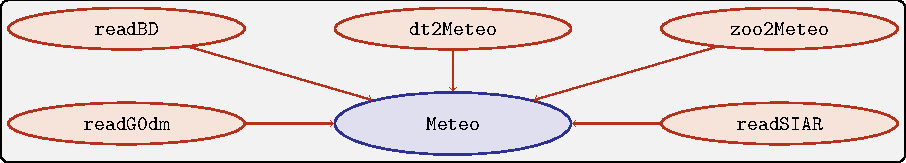
\includegraphics[width=\textwidth]{../figuras/meteo.pdf}
\end{center}
\end{frame}
\begin{frame}[label={sec:org6664b82},fragile]{\texttt{calcG0}}
 \begin{center}
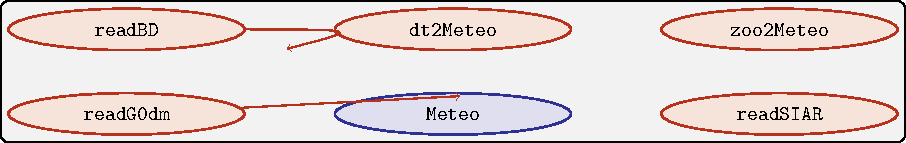
\includegraphics[width=\textwidth]{../figuras/calcg0.pdf}
\end{center}
\end{frame}
\begin{frame}[label={sec:org08115d4},fragile]{\texttt{calcGef}}
 \begin{center}
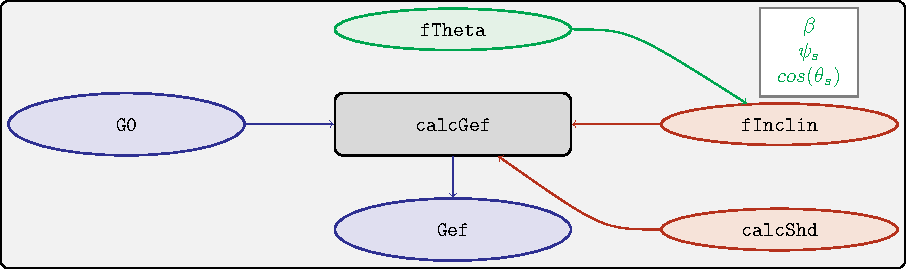
\includegraphics[width=\textwidth]{../figuras/calcgef.pdf}
\end{center}
\end{frame}
\begin{frame}[label={sec:orgc784978},fragile]{\texttt{prodGCPV}}
 \begin{center}
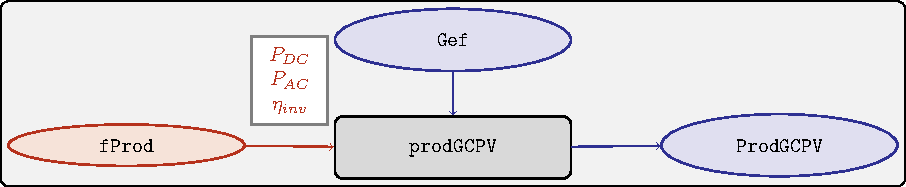
\includegraphics[width=\textwidth]{../figuras/prodgcpv.pdf}
\end{center}
\end{frame}
\begin{frame}[label={sec:org86fbec6},fragile]{\texttt{prodPVPS}}
 \begin{center}
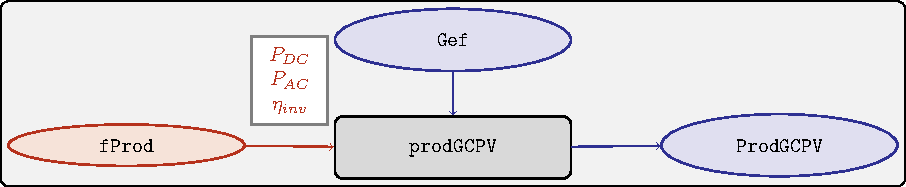
\includegraphics[width=\textwidth]{../figuras/prodpvps.pdf}
\end{center}
\end{frame}
\section{Ejemplo práctico de aplicación}
\label{sec:org48e2126}
\begin{frame}[label={sec:org83fec4d},fragile]{Información meteorológica}
 \begin{lstlisting}[numbers=left,language=r,label= ,caption= ,captionpos=b]
etsidi_1315 <- readBDi(file = "TFG/data/PVGIS_1315.csv",
                       lat = 40.4, dates.col = "Dates",
                       format = "%Y-%m-%d %H:%M:%S")
\end{lstlisting}
\end{frame}

\begin{frame}[label={sec:orga168ce6}]{Información meteorológica}
\begin{center}
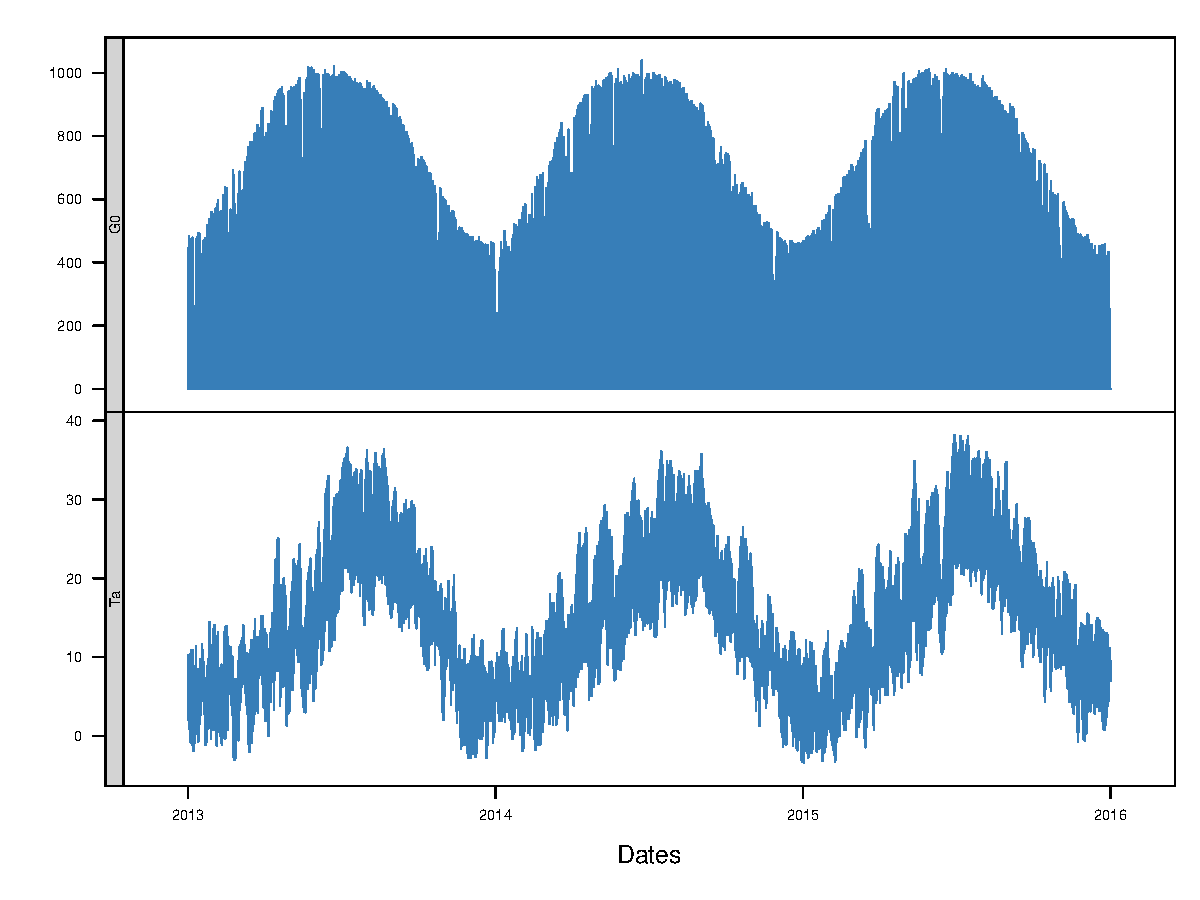
\includegraphics[height=0.9\textheight]{../figuras/ejemplos3.pdf}
\end{center}
\end{frame}
\begin{frame}[label={sec:org6eaf176},fragile]{Producción de diferentes sistemas}
 \begin{lstlisting}[numbers=left,language=r,label= ,caption= ,captionpos=b]
prod1 <- prodGCPV(lat = 40.4, modeTrk = 'fixed', modeRad = 'bdI',
                  dataRad = etsidi_1315, beta = 30, alpha = -19,
                  module = module1, generator = generator1,
                  inverter = inverter)
show(as.data.tableY(prod1))
\end{lstlisting}

\begin{verbatim}
   Dates      Eac      Edc       Yf
   <int>    <num>    <num>    <num>
1:  2013 1681.077 1757.235 1343.449
2:  2014 1698.613 1775.426 1357.463
3:  2015 1749.536 1828.569 1398.158
\end{verbatim}


\begin{lstlisting}[numbers=left,language=r,label= ,caption= ,captionpos=b]
prod2 <- prodGCPV(lat = 40.4, modeTrk = 'fixed', modeRad = 'bdI',
                  dataRad = etsidi_1315, beta = 30, alpha = -19,
                  module = module2, generator = generator2,
                  inverter = inverter)
show(as.data.tableY(prod2))
\end{lstlisting}

\begin{verbatim}
   Dates      Eac      Edc       Yf
   <int>    <num>    <num>    <num>
1:  2013 1451.873 1517.779 1319.225
2:  2014 1464.483 1530.833 1330.683
3:  2015 1506.544 1574.704 1368.901
\end{verbatim}
\end{frame}

\begin{frame}[label={sec:org2bd95d4}]{Comparación de producciones}
\begin{center}
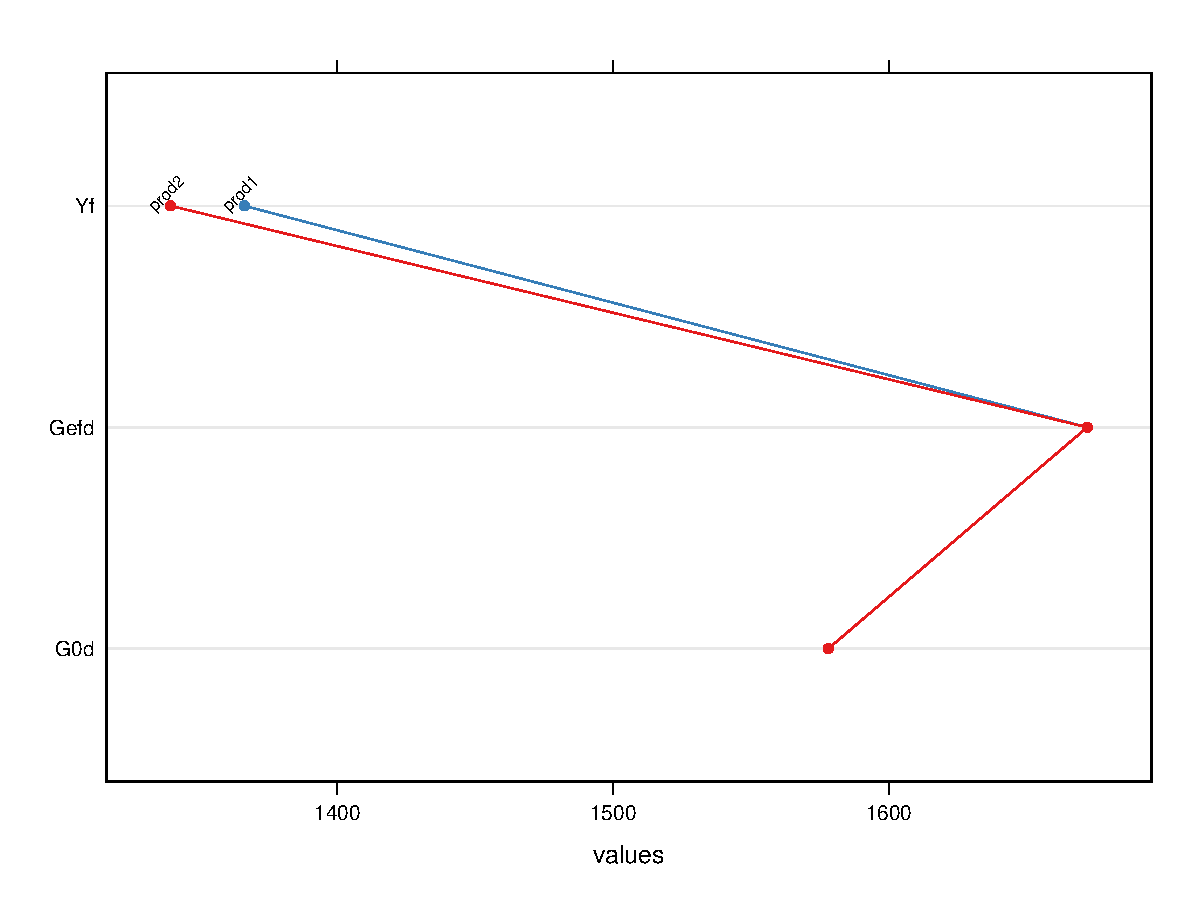
\includegraphics[height=0.9\textheight]{../figuras/ejemplos4.pdf}
\end{center}
\end{frame}
\section{Conclusiones}
\label{sec:org29bdb55}
\subsection{Aportaciones}
\label{sec:org960df63}
\begin{frame}[label={sec:orgd989ab6}]{Blame}
\begin{center}
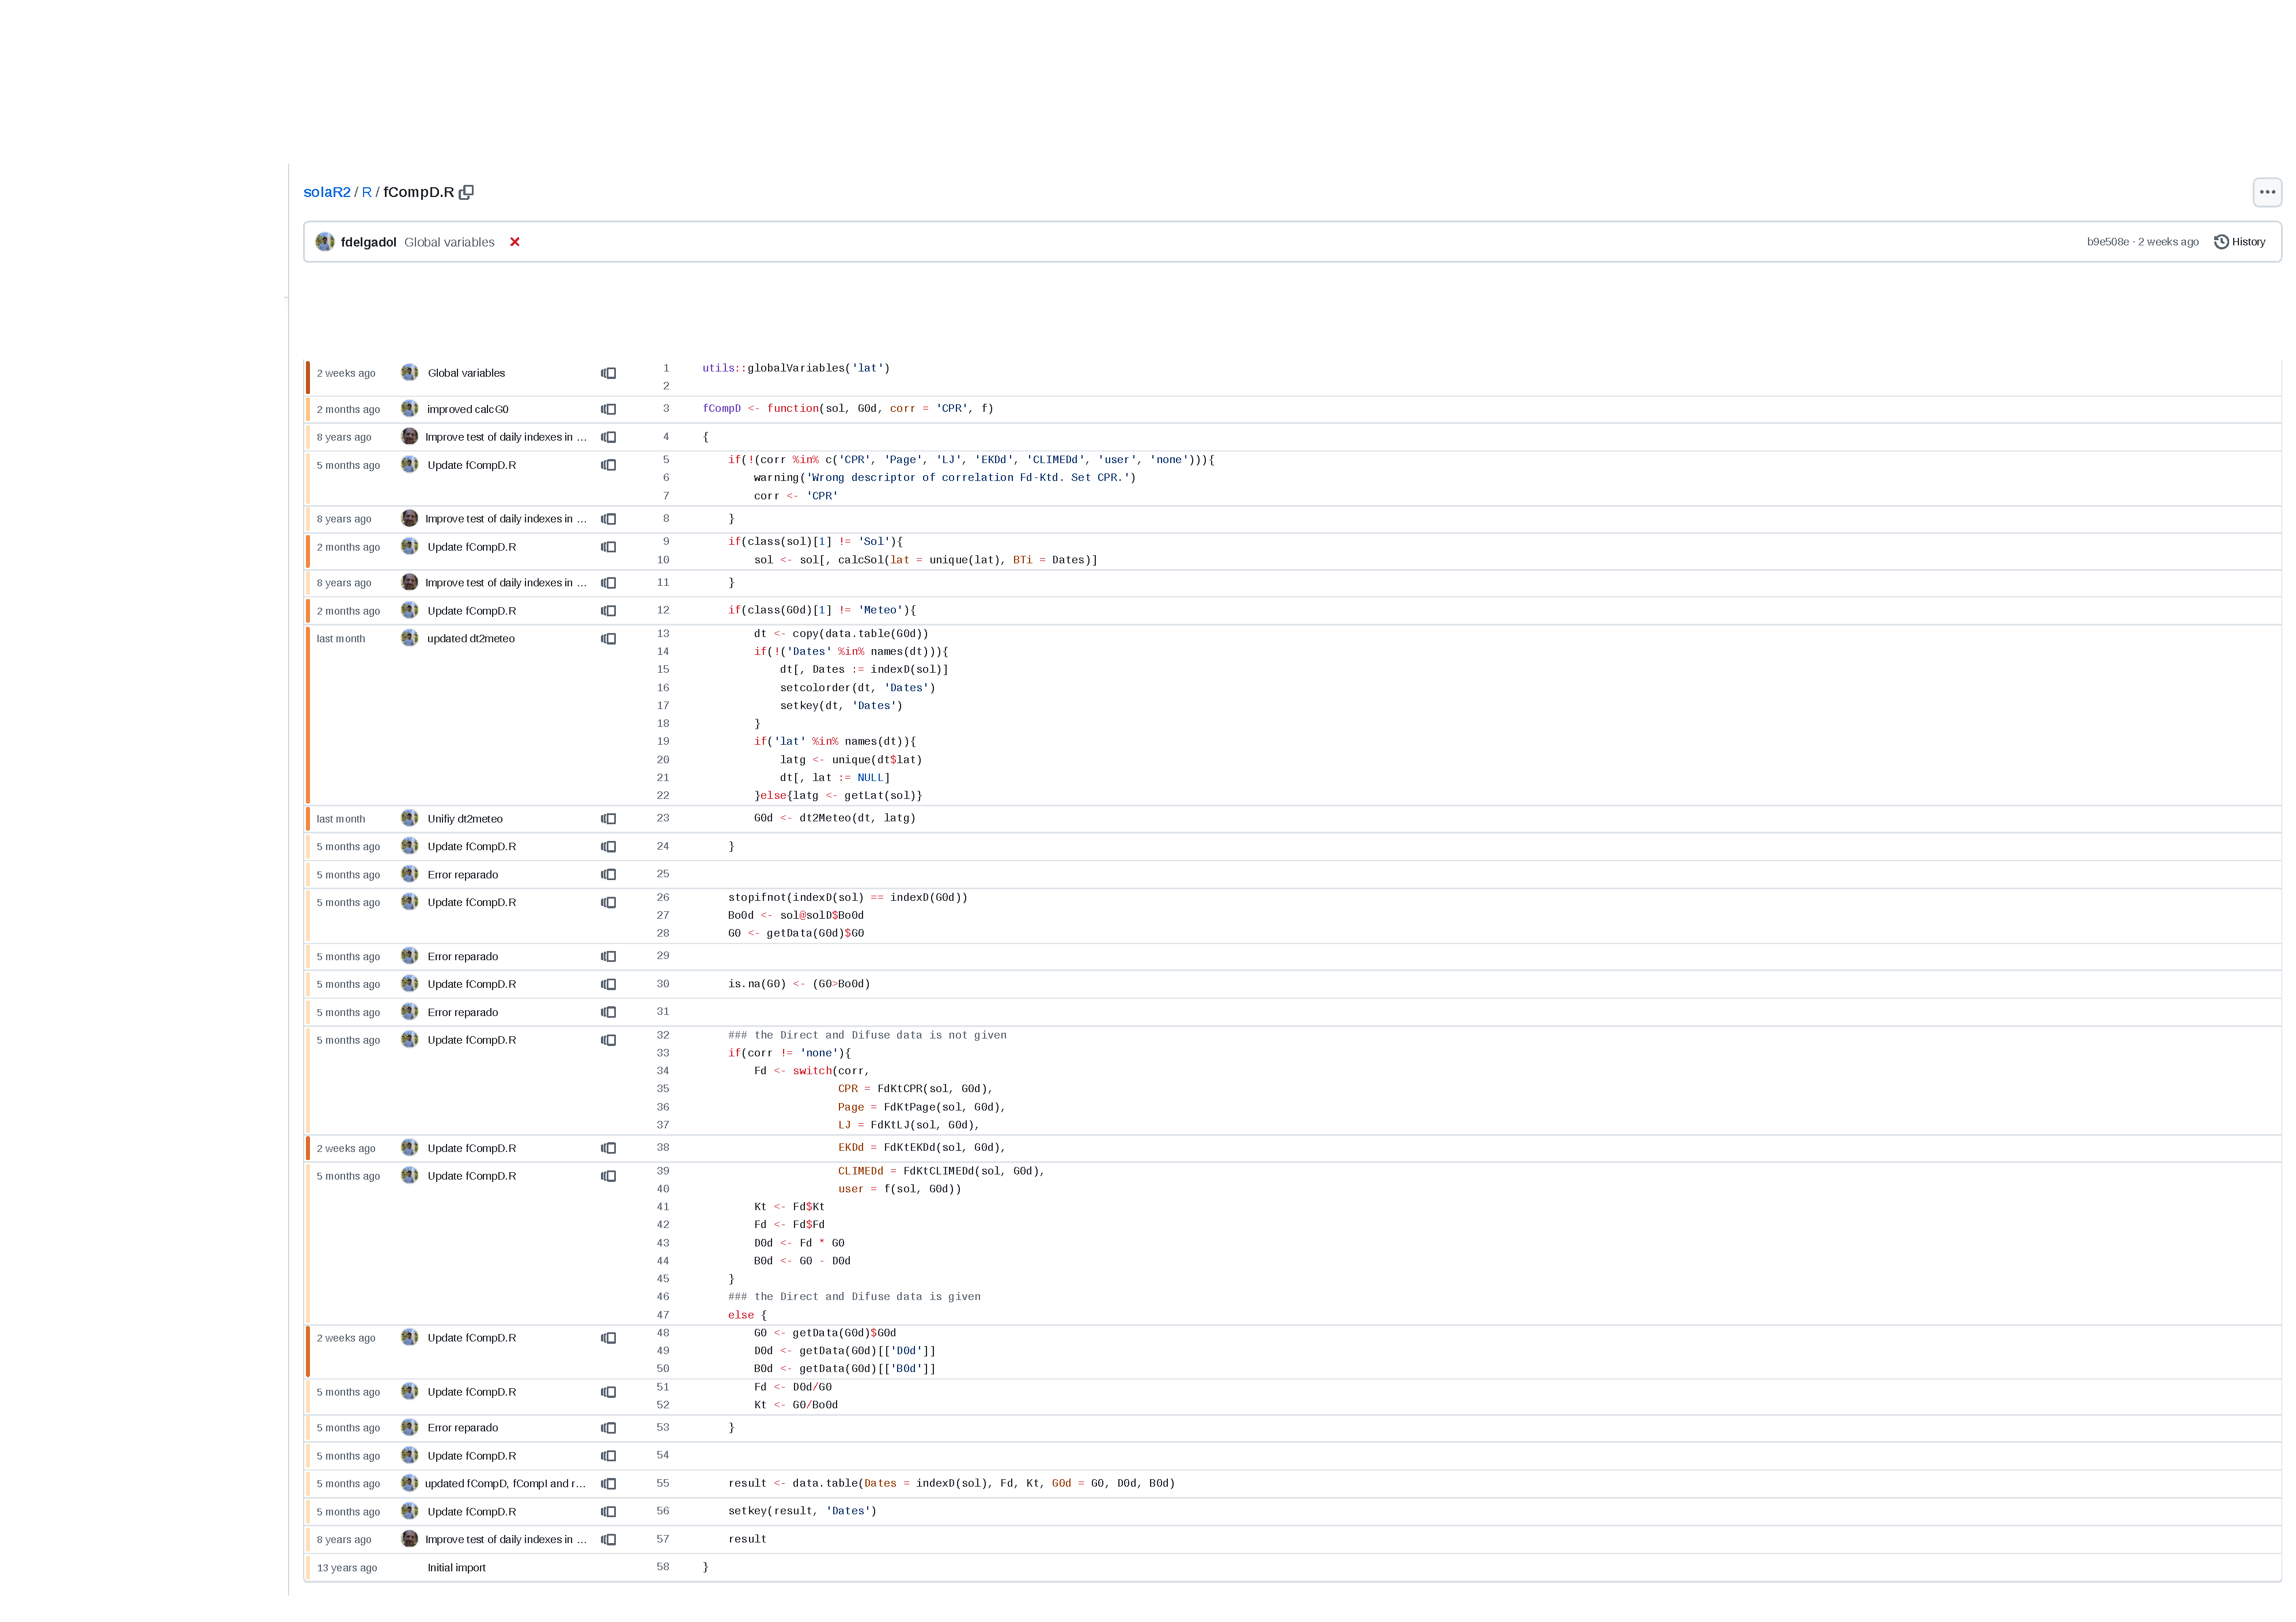
\includegraphics[height=0.9\textheight]{../figuras/blame-fCompD.pdf}
\end{center}
\end{frame}
\begin{frame}[label={sec:orgd6077de}]{Blame}
\begin{center}
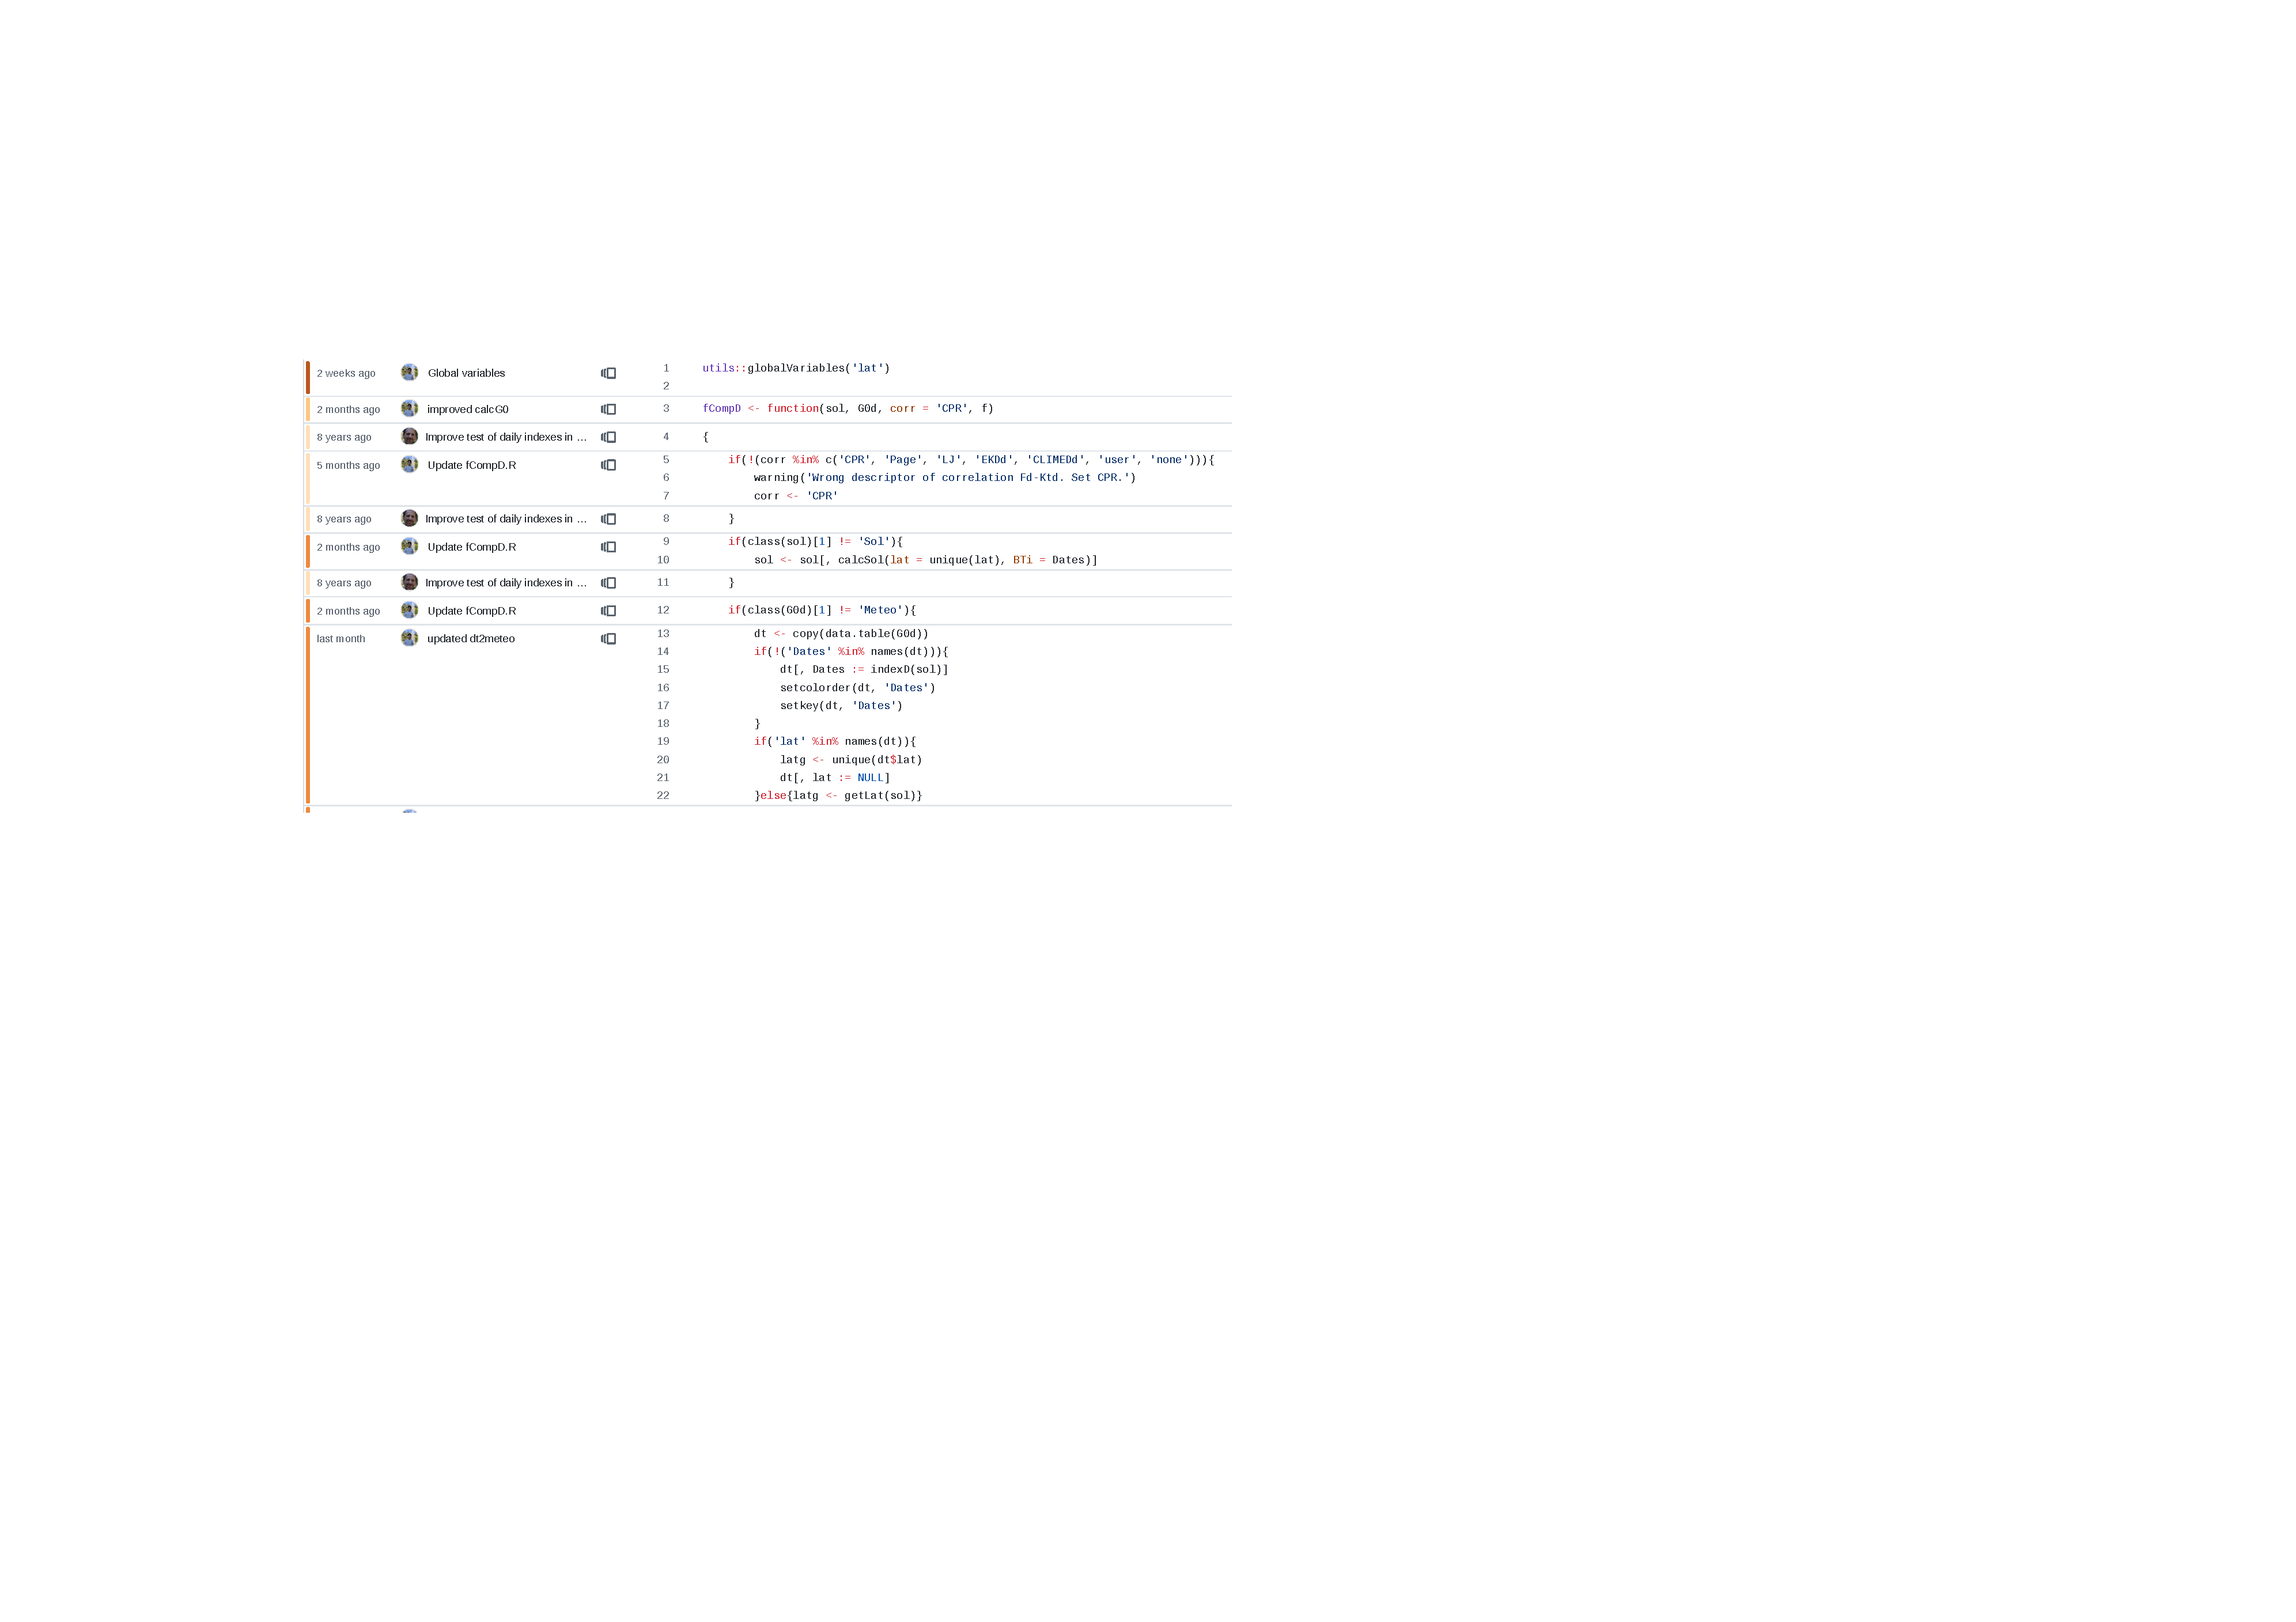
\includegraphics[width=\textwidth]{../figuras/blame-fCompD_cropped.pdf}
\end{center}
\end{frame}
\begin{frame}[label={sec:org854e4f6}]{Insights}
\begin{center}
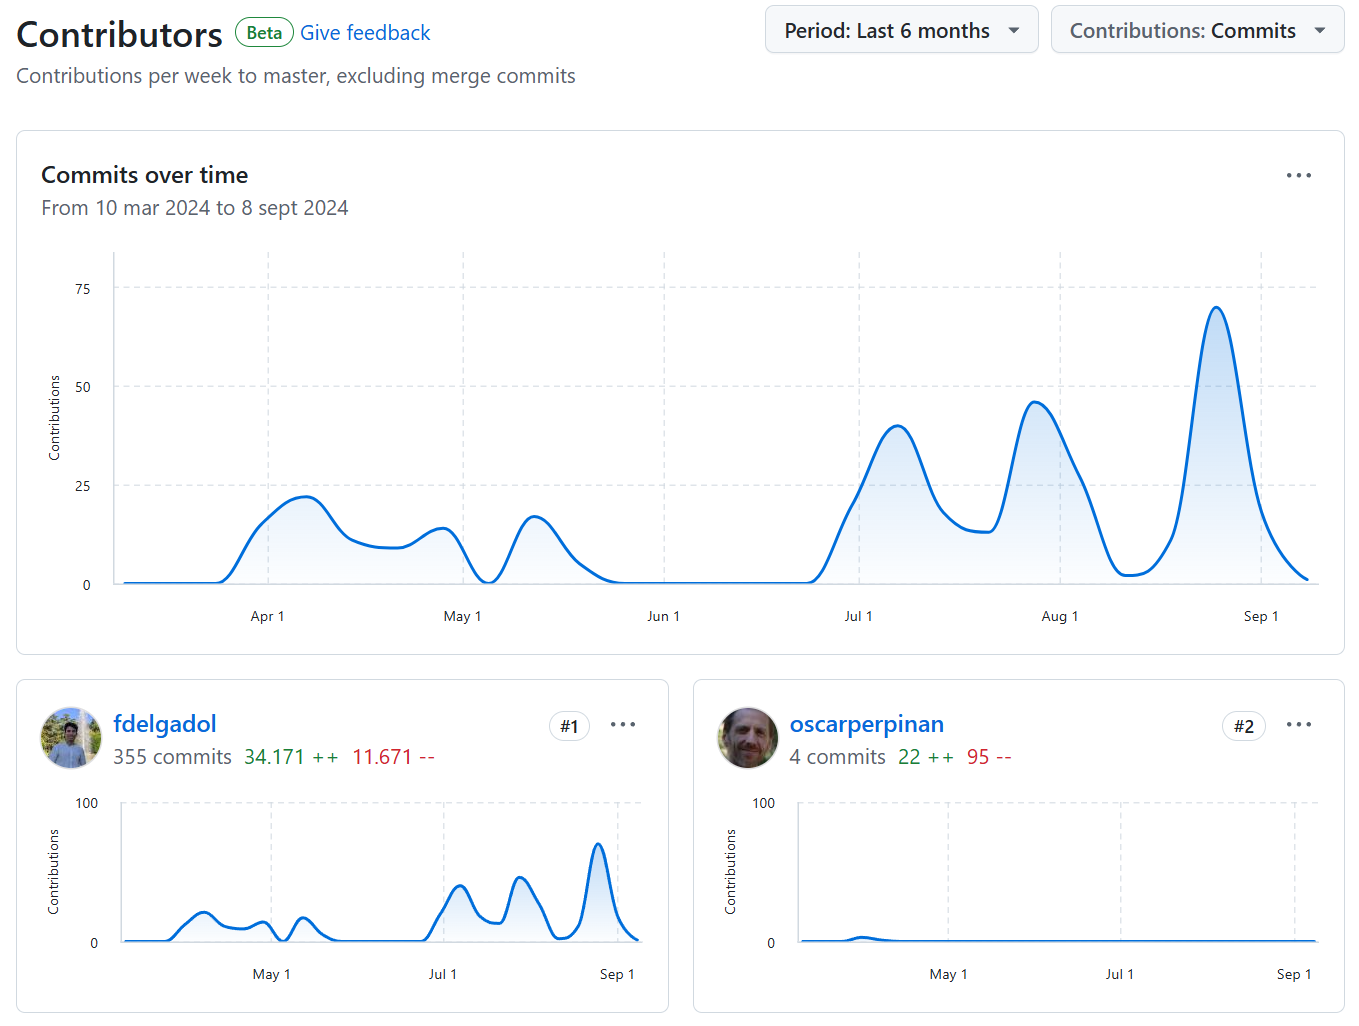
\includegraphics[height=0.9\textheight]{../figuras/contributors.png}
\end{center}
\end{frame}
\subsection{Desarrollo a futuro}
\label{sec:orgb89d7e3}
\begin{frame}[label={sec:org9680a3c},fragile]{Desarrollo a futuro}
 \begin{block}{Interfaz de usuario}
\end{block}
\begin{block}{Mejora de funciones}
\end{block}
\begin{block}{Toma de datos}
\end{block}
\begin{block}{Uso de paquete especializados en datos espaciales}
\begin{itemize}
\item \texttt{terra}
\end{itemize}
\end{block}
\end{frame}
\end{document}
